\begin{enumerate}[label=\thesection.\arabic*.,ref=\thesection.\theenumi]
\numberwithin{equation}{enumi}
\item
Sketch direct and inverse polar plots for a unity feedback system with open loop transfer function
\begin{align}
G(s) = \frac{1}{s(1+s)^2}
\end{align}
\\
\solution  
For Unity feedback system, given the open loop transfer function
\begin{align}
G(s) = \frac{1}{s(1+s)^2}
\end{align}
Now, Polar plot is defined as:
The plot of points(represented as $r.e^{\j\phi}$) obtained by varying w from 0 to $\infty$  where 
\begin{align}
r=|H(\j\omega)||G(\j\omega)|
\end{align}
\begin{align}
\phi=\angle H(\j\omega)G(\j\omega)
\end{align}
\linebreak
Inverse Polar plot is similar, in this we have;
\begin{align}
r=\frac{1}{|H(\j\omega)||G(\j\omega)|}
\end{align}
\begin{align}
\phi=-\angle H(\j\omega)G(\j\omega)
\end{align}   
The system we're analysing is unity feedback which means $H(\j\omega) = 1$
Therefore ;
%\begin{align}
%|H(\j\omega)||G(\j\omega)| = |1|.\frac{1}{|\j\omega||(1+\j\omega)^2|}  
%\end{align}
\begin{align}
|H(\j\omega)||G(\j\omega)| = \frac{1}{\omega(1+\omega^2)}
\label{eq:mod_G}
\end{align}
and Phase;
%\begin{align}
%H(\j\omega)G(\j\omega) = 1.e^{0}.1.e^{0}.\frac{1}{\omega.e^{\pi/2}} . \cbrak{\frac{1}{\sqrt{1^2 + \omega^2} . e^{tan^{-1}(\omega)}}}^2  
%\end{align}
%\begin{align}
%H(\j\omega)G(\j\omega) = 1.e^{0}.1.e^{0} \omega^{-1}.e^{-\pi/2}. (1^2 + \omega^2)^{-1} . e^{-2tan^{-1}(\omega)}  
%\end{align}
\begin{align}
\angle H(\j\omega)G(\j\omega) = \frac{-\pi}{2} - 2tan^{-1}(\omega)  
\label{eq:phase_G}
\end{align}

The following code plots the polar and inverse polar plots 
%Fig. \ref{fig:sec_order}
\begin{lstlisting}
codes/ee18btech11002/polarplot.py
\end{lstlisting}
\begin{figure}
\centering
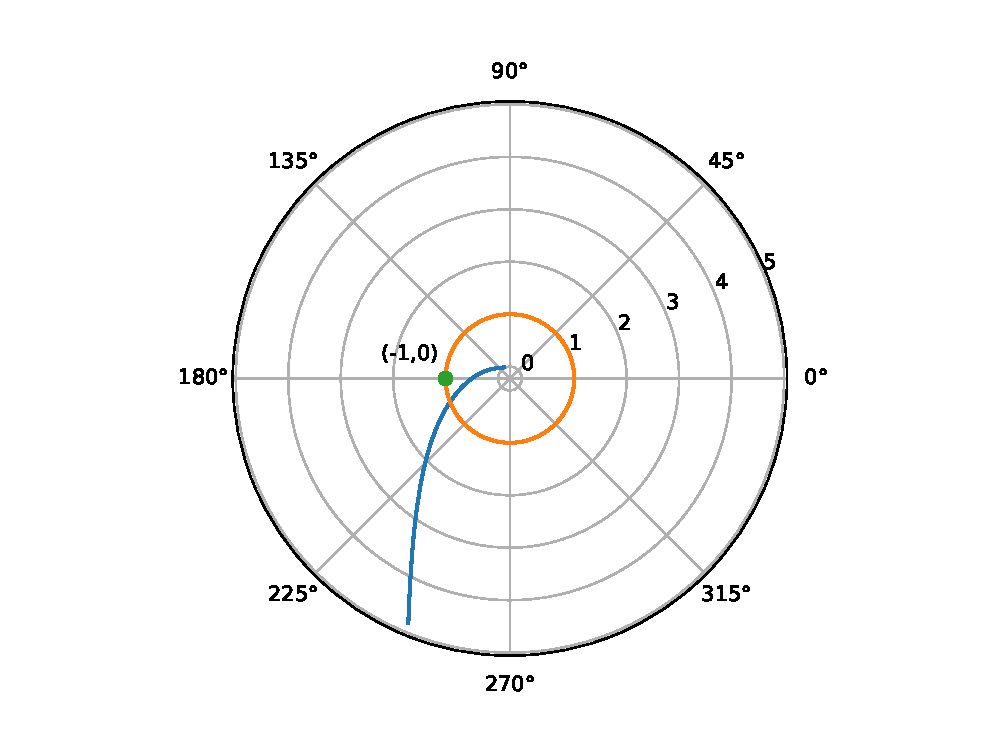
\includegraphics[width=\columnwidth]{./figs/ee18btech11002(a).eps}
\caption{Polar Plot}
\label{fig:polar_plot}
\end{figure}
\begin{figure}
\centering
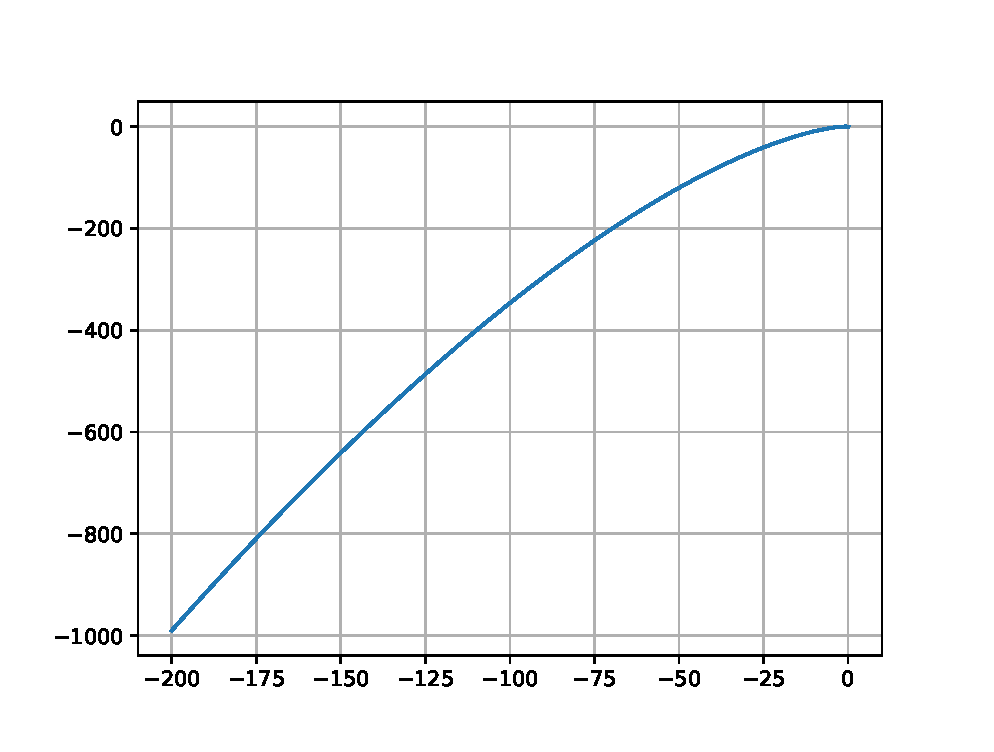
\includegraphics[width=\columnwidth]{./figs/ee18btech11002(b).eps}
\caption{Inverse Polar Plot}
\label{fig:inverse_polar_plot}
\end{figure}
\item Find the frequency at which $|G(\j\omega)| = 1$ and corresponding phase angle $\angle G(\j\omega)$
\\
\solution 
For $|G(\j\omega)| = 1$
\begin{align}
\frac{1}{\omega(1+\omega^2)} = 1
\end{align}
\begin{align}
\omega + \omega^3 - 1 = 0
\end{align}
and for the corresponding phase
\begin{align}
\angle G(\j\omega) = \frac{-\pi}{2} - 2tan^{-1}(\omega)
\end{align}
The following code calculates the value of w and $\angle G(\j\omega)$
\begin{lstlisting}
codes/ee18btech11002/solution.py
\end{lstlisting}
%\lstinputlisting{./}
%the attached code gives us the solution for the equation
and we get 
\begin{align}
\omega = 0.682
\end{align}
\begin{align}
\angle G(\j\omega)=-\frac{52}{59}\pi
\end{align}
\end{enumerate}
